%!TEX root = FreeRtos ARM uController.tex
\pagebreak
\subsection{Einrichten und Konfiguration}
\label{sec:Einrichtung und Konfiguration}
Ausgangspunkt für die nachfolgenden Codebeispiele ist die derzeit aktuelle Entwicklungsumgebung Eclipse Neon. Diese wird in der C/C++ Variante (CDT) auf dem Entwicklungssystem (Windows 7 Professional) installiert. Im Anschluss muss das GNU ARM Plugin für Eclipse CDT installiert werden, dies ist entweder über den Pluginmanager oder über den folgenden Link erhältlich: 
\newline
\newline
http://gnuarmeclipse.github.io/
\newline
\newline
Das Plugin ermöglicht die Einbindung und die Konfiguration von ARM Cross Compilern. Des Weiteren stellt es einige Beispielprojekte für ARM uController zur Verfügung. Nach der Installation des ARM Plugins, müssen die GCC ARM Toolchain und die GNU Build Tools installiert werden. 
Die Toolchain kann hier heruntergeladen werden: 
\newline
\newline
https://launchpad.net/gcc-arm-embedded
\newline
\newline
Die Toolchain und die Buildtools stellen nötigen Anwendungen die zum Compilieren und Debuggen der C und C++ Files benötigt werden. Zur Toolchain gehören unter anderem GCC als Cross Compiler und GDB (GNU Debugger) zum Debuggen der Anwendung auf der Zielplattform. GNU Buildtools beinhalte make und rm, die zum Organisieren des Builds benötigt werden. Nach der Installation müssen die Verzeichnisse der Toolchain und der Buildtools im Plugin konfiguriert werden. Mit dieser Konfiguration ist das System nun in der Lage C und C++ Dateien für die Zielplattform zu kompilieren und als Binary File (.elf) bereitzustellen. Zum Übertragen und Debuggen der Anwendung auf dem Zielsystem wird ein ISP-Programmer für ARM benötigt. Folgende ISP-Programmer werden häufig verwendet. Diese Liste ist nicht vollständig und stellt auch keine Empfehlung dar. 
\begin{itemize}
	\item Segger J-Link:
	\newline
	https://www.segger.com/jlink-debug-probes.html
	\item Keil Ulink: 
	\newline
	http://www2.keil.com/mdk5/ulink
	\item STM ST-Link/VL: 
	\newline
	http://www.st.com/en/development-tools/st-link-v2.html
\end{itemize}
Zur Nutzung des ISP müssen die benötigten Treiber und On-Chip Debugger des Herstellers installiert werden.            
Nachdem die Basiskonfiguration abgeschlossen ist, kann nun eine Basis Projekt erstellt werden. Hierfür verwendet man am Besten ein Templateprojekt des GNU ARM Plugins, siehe Abbildung \ref{fig:NewProj}.
\begin{figure}[htb]
	\centering
		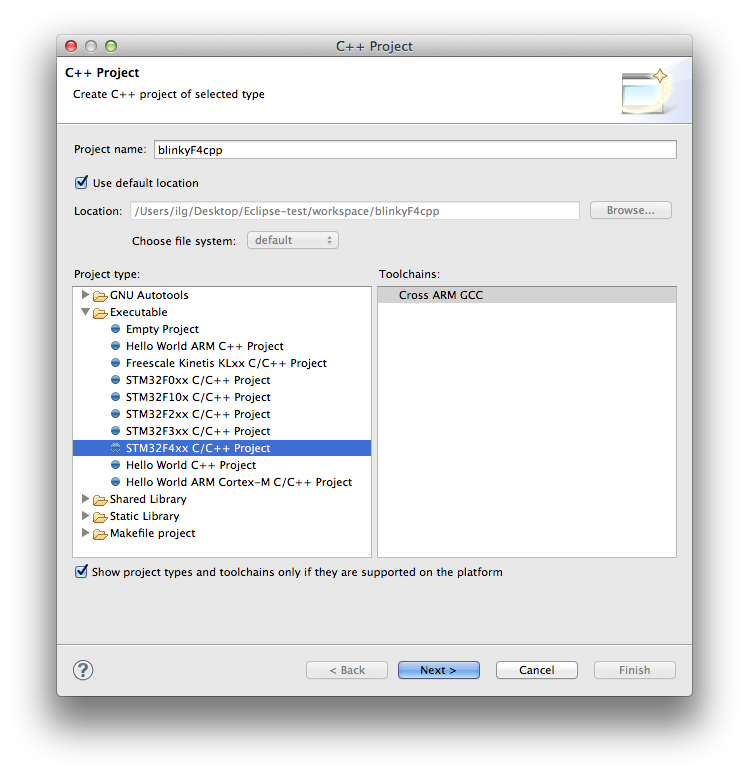
\includegraphics[width=0.4\textwidth]{Pictures/Einrichtung/NewF4Project.png}
	\caption{Erstellung eines Basisprojekts für den STM32F4 durch das GNU ARM Plugin.}
	\label{fig:NewProj}
\end{figure}
Das Templateprojekt beinhaltet bereits alle benötigten Hardware Librarys wie die STM HAL (siehe Abschnitt \ref{sec:Zielsysteme}) oder das ARM CMSIS (Cortex Microcontroller Software Interface Standard).
\begin{figure}[htb]
	\centering
		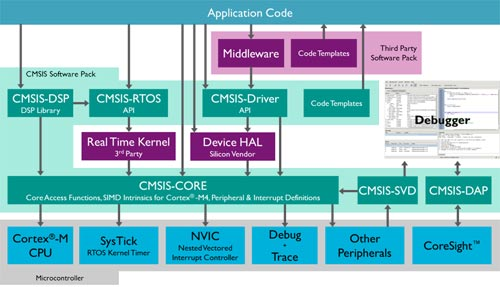
\includegraphics[width=0.4\textwidth]{Pictures/Einrichtung/CMSISv4_small.jpg}
	\caption{CMSIS}
	\label{fig:CMSIS}
\end{figure}
Das Templateprojekt sollte jetzt kompilieren und mittels ISP-Programmer auf auf dem Zielsystem ausgeführt werden können.
Als nächstes wird FreeRTOS in das Templateprojekt eingebunden, hierfür kann auf www.freertos.org die gepackte Variante der Demoprojekte heruntergeladen werden. Für den STM32F4 stehen spezielle Cortex M4 Portierungen zur Verfügung. Nach der Einbindung sollten die Verzeichnisse wie in Abbildung \ref{fig:SourceTree} aussehen.
\begin{figure}[htb]
	\centering
		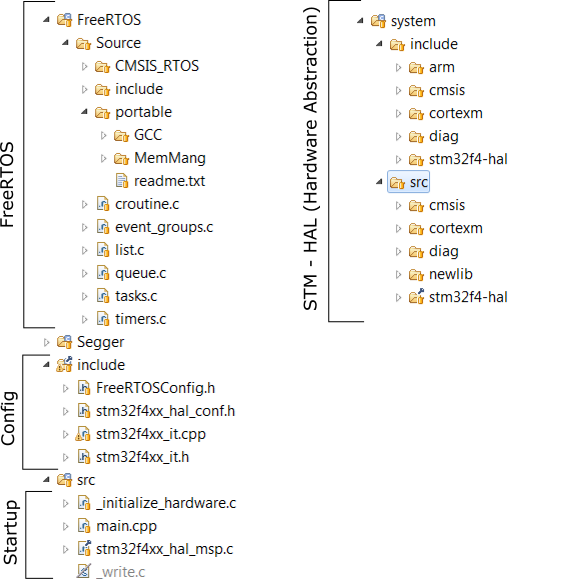
\includegraphics[width=0.4\textwidth]{Pictures/Einrichtung/sourceTree.png}
	\caption{Source}
	\label{fig:SourceTree}
\end{figure}

